% Name: Dumbbell chart
% Description: Mean test scores in five topics before and after a course, a gray dot and a blue dot on each row joined by a bar whose length is the gain.
% Tags: dumbbell chart, before and after, comparison, change

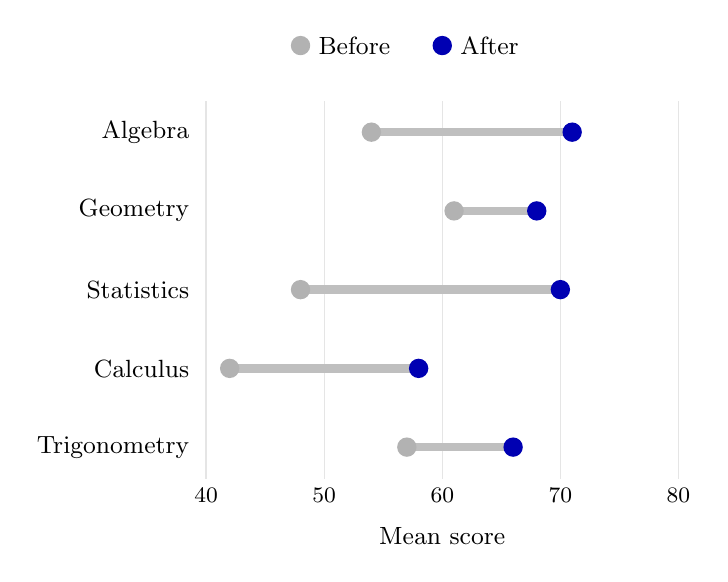
\begin{tikzpicture}[font=\small, x=0.15cm]
  % Scores run from 40 to 80; x = 0 is a score of 40.
  \foreach \v in {40,50,...,80} {
    \draw[gray!20] (\v-40,-0.4) -- (\v-40,4.4);
    \node[below, font=\footnotesize] at (\v-40,-0.4) {\v};
  }
  \node[below=14pt] at (20,-0.4) {Mean score};
  \foreach \name/\a/\b [count=\i from 0] in {Algebra/54/71, Geometry/61/68, Statistics/48/70, Calculus/42/58, Trigonometry/57/66} {
    \draw[gray!50, line width=3pt] (\a-40,4-\i) -- (\b-40,4-\i);
    \fill[gray!60] (\a-40,4-\i) circle (3.5pt);
    \fill[blue!70!black] (\b-40,4-\i) circle (3.5pt);
    \node[left] at (-0.6,4-\i) {\name};
  }
  \fill[gray!60] (8,5.1) circle (3.5pt) node[right=3pt, black] {Before};
  \fill[blue!70!black] (20,5.1) circle (3.5pt) node[right=3pt, black] {After};
\end{tikzpicture}
